\section{Programmazione Asincrona}

Se la necessità di eseguire più operazioni, indipendenti tra loro, in \textbf{parallelo} porta
alla creazione di più thread, altre esigenze di programmazione possono beneficiare
di un approccio differente.

L'uso dei thread trova piena giustificazione quando occorre eseguire algoritmi complessi, basati
principalmente sull'uso intenso della CPU e si dispone di un hardware multicore.

In queste situazioni, infatti, è possibile ridurre il tempo complessivo di elaborazione sfruttando il fatto
che più computazioni procedono parallelamente.

Se il programma, invece, deve coordinare molteplici attività che si svolgono \textbf{al di
  fuori} di esso, il problema dominante diventa l'attesa dei risultati.
Sebbene sia possibile gestire queste situazioni creando più thread, questo, in generale, non è
conveniente.

\subsection{Concorrenza non è parallelismo}
\begin{itemize}
  \item \textbf{Parallelismo}: più computazioni procedono fisicamente nello stesso istante
        \begin{itemize}
          \item Richiede più unità di calcolo (core): permette di ridurre il tempo di elaborazione per attività CPU-
                bound
          \item Lo strumento naturale in Rust è il thread
        \end{itemize}
  \item \textbf{Concorrenza}: più compiti progrediscono in modo interlacciato, non necessariamente simultaneo
        \begin{itemize}
          \item Un singolo core può gestire migliaia di compiti concorrenti se
                ognuno passa gran parte del tempo in attesa
          \item Il vantaggio non è la velocità di calcolo, ma la capacità di
                sovrapporre molte attese: un unico thread può coordinare migliaia di attese
        \end{itemize}
\end{itemize}


\section{Operazioni bloccanti attese}

Molte operazioni richiedono di ottenere informazioni da un \textbf{sottosistema separato}, come ad esempio
il file system, la rete, un timer, etc.

Per queste operazioni l'esecuzione non può proseguire finché la risposta non è disponibile.
Il sistema operativo rileva la situazione e sposta il thread corrente nello stato
"\textit{NotRunnable}", sospendendolo, e la CPU viene liberata, ma lo stack dei thread
\textbf{resta allocato} per tutta la durata dell'attesa.

La \textbf{domanda di progetto}: : il collo di bottiglia è la CPU o l'attesa (I/O, rete, timer)?

\begin{itemize}
  \item CPU-bound $\rightarrow$ parallelismo con thread
  \item I/O-bound $\rightarrow$ concorrenza con esecuzione asincrona
\end{itemize}


\begin{tcolorbox}
  \textbf{Nota:} Si usano i \textbf{thread} quando \textbf{occorre elaborare} in
  parallelo, mentre si usa l'\textbf{esecuzione asincrona}
  quando \textbf{occorre aspettare} in parallelo
\end{tcolorbox}

\subsection{Il costo dei thread}

Ogni thread del sistema operativo ha un costo fisso, indipendente dal lavoro che
svolge:

\begin{itemize}
  \item \textbf{Stack pre-allocato}: tipicamente da 1 a 8 MB di spazio di indirizzamento riservato per thread
  \item \textbf{Strutture del kernel}: descrittore del thread, slot nello schedulatore, contabilità
  \item \textbf{Cambio di contesto}: salvataggio/ripristino dei registri, invalidazione di cache e TLB ($\sim\,1-2\,\mu s$)
\end{itemize}

Finché i thread sono poche decine, questi costi sono trascurabili, iventano
critici quando se ne vogliono creare molti (1000+), come in un server di rete
Esempio: 10.000 connessioni simultanee con un thread ciascuna \(\to \) diversi
GB solo di stack.
Si paga il costo di un thread completo per fargli fare, di fatto, nulla


\section{Tre strategie di esecuzione}

Se il programma ha altro da fare durante l'attesa, ci sono tre strategie possibili:


\begin{table}[h!]
  \renewcommand{\arraystretch}{1.6}
  \centering
  \begin{tabularx}{\textwidth}{>{\raggedright\arraybackslash}X >{\raggedright\arraybackslash}X >{\raggedright\arraybackslash}X >{\raggedright\arraybackslash}X}
    \toprule
    \textbf{Strategia}                    & \textbf{Idea}                                 & \textbf{Vantaggi}                                            & \textbf{Limiti}                                                        \\
    \midrule
    Sequenziale \newline (bloccante)      & Aspetto e poi continuo                        & Semplice \newline Facile da ragionare                        & Spreca tempo di CPU \newline Nessuna sovrapposizione                   \\
    \midrule
    Thread multipli \newline (preemptive) & Delego l'operazione bloccante ad altri thread & Parallelismo reale \newline Sfrutta multicore                & Costo elevato (stack, scheduling) \newline Sincronizzazione complessa  \\
    \midrule
    Asincronia \newline (cooperativo)     & Separo richiesta e continuazione              & Non blocca il thread \newline Scala a migliaia di operazioni & Più complesso concettualmente \newline Richiede supporto di esecuzione \\
    \bottomrule
  \end{tabularx}
\end{table}



\begin{figure}[h!]
  \centering
  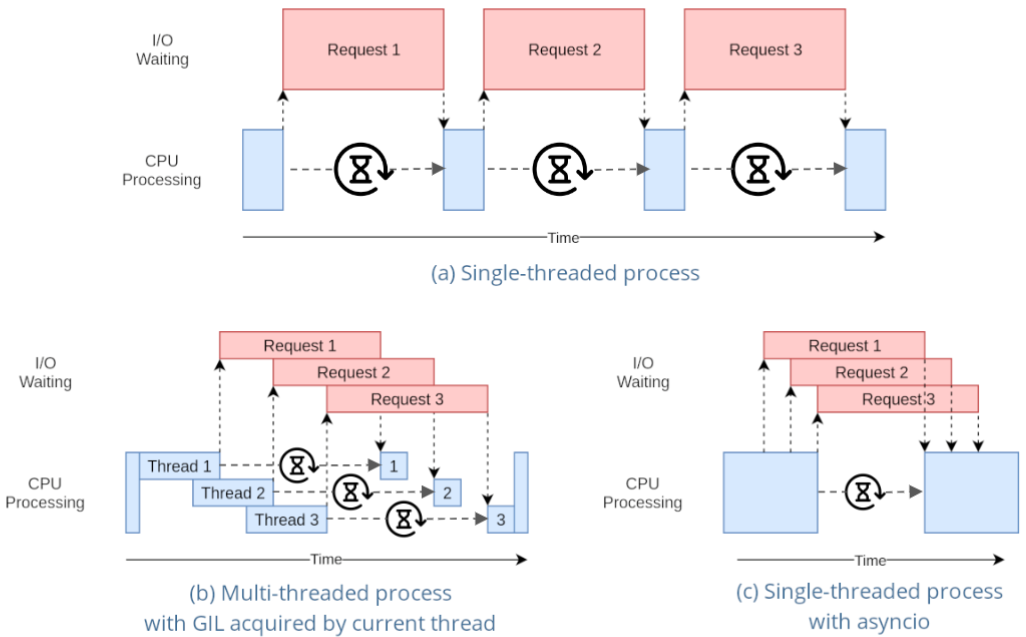
\includegraphics[width=0.8\linewidth]{content/API_Programming/images/2026-05-22-20-49-01.png}
\end{figure}



% \begin{flushleft}
%   \begin{minipage}{0.65\linewidth}
%     \raggedright
%     Se il programma deve svolgere altri compiti, oltre a quello che ha generato l'attesa,
%     si creano tre possibilità:

%     \begin{itemize}
%       \item Gli altri compiti saranno eseguiti successivamente, dal thread corrente
%       \item Si creano più thread secondari per eseguirli, accollandosi la complessità legata alla loro
%             sincronizzazione
%       \item Si organizza il codice in modo tale da separare la richiesta di eseguire l'operazione dalle operazioni che
%             dovranno essere fatte quando arriverà la risposta, così da non bloccare l'esecuzione del thread
%             corrente, ammesso che vi sia altro da fare
%     \end{itemize}
%   \end{minipage}%
%   \hfill
%   \begin{minipage}{0.3\linewidth}
%     \centering
%     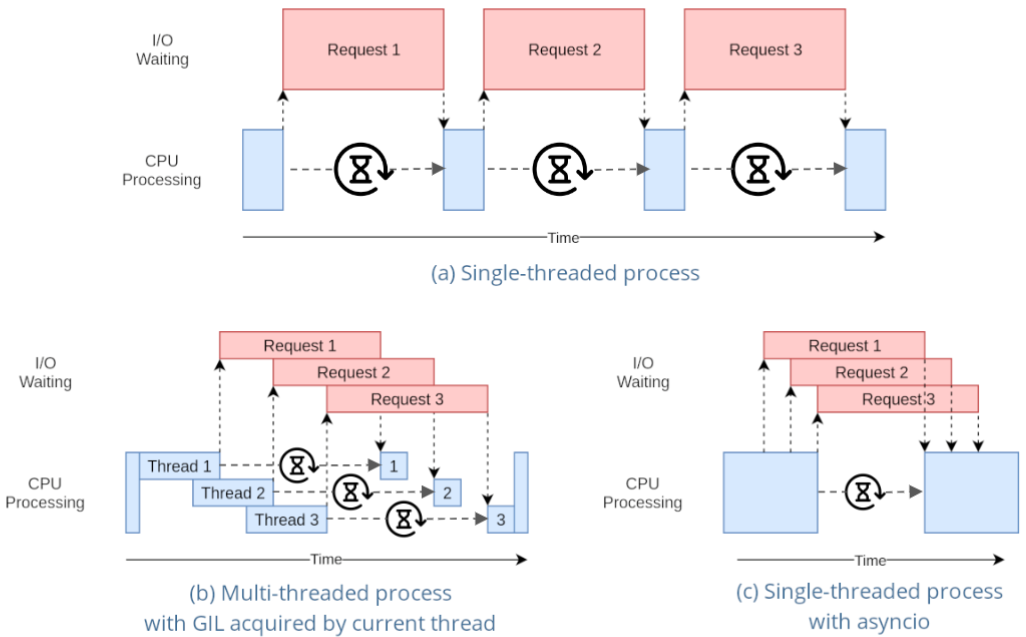
\includegraphics[width=\linewidth]{content/API_Programming/images/2026-05-22-20-49-01.png}
%   \end{minipage}
% \end{flushleft}


\section{Separare richiesta e continuazione (callback)}

\paragraph{Nell'approccio asincrono}: avvio un'operazione, NON attendo il risultato, speficico cosa fare quando il risultato arriva (continuazione)

Il modo più semplice per indicare la continuazione è una callback. Pseudo-codice:

\mintinline{rust}!read_async(file, |result| { process(result); });!

Timeline

\begin{enumerate}
  \item[\textit{$t_0$}]: invoco \mintinline{rust}|read_async(...)|
  \item[\textit{$t_1$}]: il programma continua
  \item[\textit{$t_2$}]: arriva il risultato
  \item[\textit{$t_3$}]: viene eseguita la callback
\end{enumerate}

In Javascript è semplice perché funziona single-threaded by design con una message queue.
In Rust non abbiamo una message queue, il programmatore si sceglie cosa fare utilizzando
tre librerie diverse come Tokio, smol o async-std.

\begin{tcolorbox}
  \textbf{Vantaggio:} il thread NON resta bloccato dall'attesa e può svolgere altro lavoro
\end{tcolorbox}




% \section{Esecuzione asincrona}




% Il modo più diretto di implementare la terza strategia richiede che le azioni conseguenti
% ad una data operazione bloccante siano racchiuse in un'apposita funzione (callback).
% Tale funzione riceve come parametro il risultato dell'operazione bloccante e sarà invocata quando il
% sottosistema che è stato interrogato avrà fornito la propria risposta.

% Chi si occupa di fornire tale valore e in quale thread avverrà la chiamata?
% Linguaggi diversi offrono soluzioni alternative.

% \begin{flushleft}
%   \begin{minipage}{0.65\linewidth}
%     \raggedright
%     \paragraph{Funzionamento in Javascript}

%     In Javascript, ad esempio, il modello di esecuzione prevede la presenza di una coda dei
%     messaggi, in cui il driver del sottosistema interrogato provvede ad inserire il risultato

%     \begin{itemize}
%       \item Il driver è eseguito in un thread separato
%       \item Il thread principale esegue costantemente un ciclo, in cui attende la presenza di un messaggio, lo estrae dalla coda e lo elabora
%       \item Quando la risposta arriverà, questa verrà naturalmente elaborata dal ciclo di elaborazione dei messaggi
%     \end{itemize}
%   \end{minipage}%
%   \hfill
%   \begin{minipage}{0.3\linewidth}
%     \centering
%     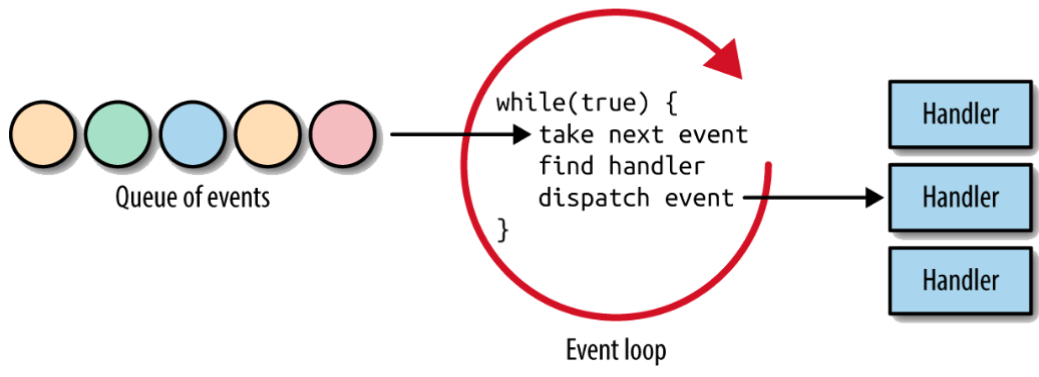
\includegraphics[width=\linewidth]{content/API_Programming/images/2026-05-22-20-58-12.png}
%   \end{minipage}
% \end{flushleft}

% \section{Continuazioni e callback}




% \begin{center}
%   \begin{minipage}{0.57\linewidth}
%     Un tipico modo per implementare operazioni asincrone è basarsi su API ad eventi.
%     Ovvero funzioni che permettono di richiedere ad uno strato soggiacente (come il
%     sistema operativo o una piattaforma di esecuzione) l'operazione che si intende
%     eseguire, passando una callback che dovrà essere invocata nel momento in cui lo
%     strato soggiacente avrà terminato la sua parte di esecuzione.

%   \end{minipage}%
%   \hfill
%   \begin{minipage}{0.4\linewidth}
%     \centering
%     \begin{minted}[breaklines]{rust}
% val f1: AsyncRead = …
% val f2: AsyncRead = …
% read_async(f1, vec![], |buffer: &[u8]|{
%   // process buffer from file1…
% });
% read_async(f2, vec![], |buffer: &[u8]|{
%   // process buffer from file2
% });
% \end{minted}
%   \end{minipage}
% \end{center}


\section{I limiti delle callback}

\begin{flushleft}
  \begin{minipage}{0.35\linewidth}
    \raggedright
    % \section{The callback hell}
    % Questo modo di scrivere il codice, tuttavia, crea grossi problemi quando
    % l'azione che si sta compiendo richiede, \textbf{in cascata}, una seconda azione asincrona.
    % Occorre infatti che la callback indicata provveda ad invocare un'ulteriore
    % operazione passando la relativa callback.

    % Le cose si complicano se tale operazione è ciclica e se occorre gestire
    % eventuali errori. Per questo motivo è spesso utile trasformare il codice
    % in una macchina a stati finiti.

    % Gli errori possono originarsi in momenti molto
    % diversi:

    % \begin{itemize}
    %   \item All'atto dell'invocazione della funzione asincrona
    %   \item Come conseguenza dell'elaborazione asincrona
    % \end{itemize}

    Ci sono tre limiti importanti legati all'uso delle callback:
    \begin{itemize}
      \item \textbf{Annidamento}: illeggibile al crescere dei passi
      \item \textbf{Errori}: in punti diversi: all'invocazione e nell'elaborazione asincrona
      \item Cicli e tentativi ripetuti richiedono una \textbf{macchina a stati} scritta a mano
    \end{itemize}

    I costrutti \verb|async|/\verb|await| automatizzano questa trasformazione


    \begin{tcolorbox}
      \textbf{Nota:} Le callback funzionano, ma non scalano in complessità
    \end{tcolorbox}
  \end{minipage}%
  \hfill
  \begin{minipage}{0.6\linewidth}
    \begin{minted}[breaklines]{rust}
let handle1 = open_file_async("f1", FileMode::read )?;
let handle2 = open_file_async("f2", FileMode::write)?;
let mut buffer = vec![];
read_async(handle1, &mut buffer, |res1|{
  if (res1.is_ok()) {
    write_async(handle2, res1.unwrap(), |res2| {
        if (res2.is_ok()) {
          //scrittura completata con successo
        } else {
          //scrittura fallita
        }
    });
  } else {
    //lettura fallita
  }
})?; // impossibilità di leggere
//Quando il programma arriva qui, non è ancora
//stato fatto nulla!
\end{minted}
  \end{minipage}
\end{flushleft}

\subsection{Async/await: stessa idea, forma diversa}


\begin{flushleft}
  \begin{minipage}[t]{0.45\linewidth}

    \paragraph{Callback}


    \raggedright
    \begin{minted}[breaklines]{rust}
read_async(…, |r1| {
  write_async(…, |r2| {
  …
  });
});
// Quando arriva qui è già successo qualcosa?
\end{minted}
  \end{minipage}%
  \hfill
  \begin{minipage}[t]{0.45\linewidth}

    \paragraph{Async/await}


    \raggedright
    \begin{minted}[breaklines]{rust}
sync {
  let r1 = read(…).await;
  let r2 = write(r1).await;
}
// Il compilatore trasforma il codice nella 
// stessa macchina a stati delle callback
\end{minted}
  \end{minipage}
\end{flushleft}

Se async/await genera una macchina a stati $\to$ chi la esegue?




% \section{Esecuzione parziale}
% Un primo passo che aiuta a semplificare il problema è provare a riscrivere la forma
% \textbf{annidata} delle callback in una forma \textbf{lineare}, appoggiandosi ad una struttura dati che
% mantenga le informazioni di stato (\textbf{future}).

% \begin{center}
%   \begin{minipage}{0.45\linewidth}
%     \begin{minted}[breaklines]{rust}
% read_async(h1, &mut buffer, |res1|{
%   if (buffer.is_ok()) {
%     write_async(h2, res1.unwrap(), |res2| {
%       if (res2.is_ok()) { /* success */ }
%       else { /* … */ }
%     });
%   } else {
%     //lettura fallita
%   }
% })?;
% \end{minted}
%   \end{minipage}%
%   \hfill
%   \begin{minipage}{0.45\linewidth}
%     \begin{minted}[breaklines]{rust}
% //buffer -> Future<Result<[u8]>>
% read_async(h1, &mut buffer)
%   .and_then( |res1|{
%     if (res1.is_ok()) {
%     write_async(h2, res1.unwrap());
%     } else { /* … */ }) //Future<Result<usize>>
%   .and_then(|res2| {
%     if (res2.is_ok()) { /* success */ }
%     else { /* … */ }
%     }) //Future<Result<()>>
%   .map_error( |err| { /* … */ });
% \end{minted}
%   \end{minipage}
% \end{center}



% \begin{center}
%   \begin{minipage}{0.65\linewidth}

%     Questa forma aiuta a vedere come le operazioni che si intendono eseguire possano
%     essere viste come una macchina a stati finiti, che evolve "a strappi".
%     Quando raggiunge uno stato intermedio ritorna e, per continuare, sarà necessario riprenderne
%     l'esecuzione passando come parametro l'esito dell'operazione asincrona che ha causato la
%     sospensione.
%   \end{minipage}%
%   \hfill
%   \begin{minipage}{0.3\linewidth}
%     \centering
%     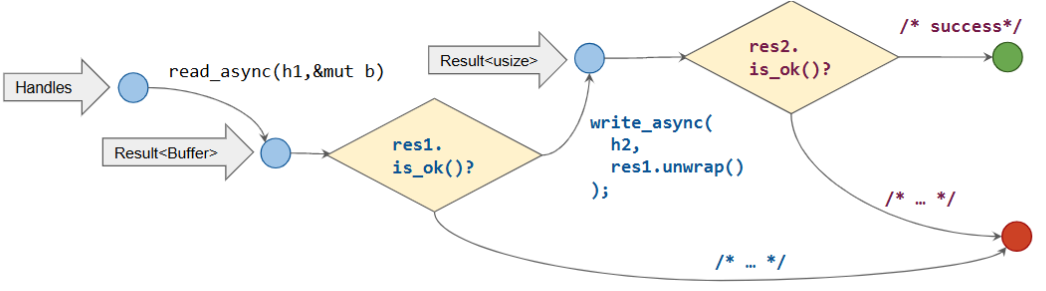
\includegraphics[width=\linewidth]{content/API_Programming/images/2026-05-22-21-20-19.png}
%   \end{minipage}
% \end{center}


% La macchina a stati finiti può essere implementata da una chiusura.
% Essa racchiude il proprio \textbf{stato} e tutte le \textbf{variabili locali} di cui l'esecuzione ha bisogno.
% Quando viene eseguita ritorna un valore che indica se ha raggiunto uno degli stati finali o se si trova
% ancora in uno stato intermedio.
% Questo permette di non bloccare il thread corrente e procedere con l'esecuzione di altri task.

% I punti di blocco sono tutti in corrispondenza degli stati intermedi.
% Questi sono immediatamente preceduti dall'invocazione di una funzione asincrona.
% Quando uno stato intermedio viene raggiunto, la chiusura ritorna.

% Perché la macchina a stati possa progredire occorrono due condizioni:

% \begin{itemize}
%   \item Che la funzione asincrona invocata scateni qualche attività (in che thread avviene?) che possa portare all'evoluzione dello stato
%   \item Che ci sia qualcuno che indichi che vi sono le condizioni affinché lo stato possa evolvere
% \end{itemize}


\newpage
\section{Funzioni asincrone}

Il compilatore Rust supporta esplicitamente la programmazione asincrona grazie
all'introduzione di due parole chiave nel linguaggio: \textbf{async} e \textbf{await}


\subsection{La parola chiave \textit{async}}

Anteporre \verb|async| a una funzione, o a un blocco, ne cambia radicalmente la
semantica

\begin{itemize}
  \item Il compilatore analizza il corpo e lo trasforma in una macchina a stati finiti
  \item Il tipo di ritorno passa da \textbf{T} a un tipo anonimo che implementa il tratto \textbf{Future<Output=T>}
  \item Il corpo della funzione viene ridotto alla sola inizializzazione di quella macchina a stati
\end{itemize}

Conseguenza cruciale: \textbf{chiamare una funzione async NON ne esegue il corpo}

\begin{itemize}
  \item Restituisce solo un \textbf{Future} inerte, nel suo stato iniziale
  \item È un valore che descrive una computazione da fare, non la computazione già avviata
\end{itemize}

\begin{minted}[breaklines]{rust}
// quello che si scrive:
async fn copy(f1: String, f2: String) -> Result<()> { /* codice */ }

// quello che il compilatore genera, concettualmente
fn copy(f1: String, f2: String) -> impl Future<Output = Result<()>> { /* SM init */ }
\end{minted}


\subsection{L'operatore \textit{.await}}

Per ottenere il risultato di un \textbf{Future}, occorre attenderlo
esplicitamente con l'operatore \verb|.await|.
Senza \verb|.await|, il Future resta inerte e non viene mai eseguito (il compilatore lo
segnala con un warning).



\paragraph{Semantica di \textit{.await}}

\begin{itemize}
  \item Se il valore non è ancora disponibile, la funzione corrente si \textbf{sospende} e restituisce il controllo
  \item Il thread non resta bloccato: è libero di eseguire altri task pronti
  \item Quando il valore arriva, l'esecuzione riprende esattamente dal punto di sospensione
\end{itemize}

Ogni \textit{.await} introduce un nuovo stato nella macchina a stati della funzione.
L'operatore \textbf{?} si combina con \textit{.await} per proparare gli errori in modo lineare.


\textit{.await} NON esegue il \textbf{Future} $\to$ segnala solo dove sospendere e riprendere.



% \section{Async e await}

% Il compilatore Rust supporta esplicitamente la programmazione asincrona grazie
% all'introduzione di due parole chiave nel linguaggio (\textbf{async} e \textbf{await}) ed alla
% presenza di un tipo specifico (\textbf{Future}) nella libreria core.

% Se una funzione o un blocco di codice sono preceduti dalla parola chiave \textbf{async}, il compilatore ne
% analizza il contenuto e lo trasforma in una macchina a stati.
% La funzione o il blocco vengono ridotti all'inizializzazione di tale macchina a stati.
% Il tipo restituito viene trasformato da \textbf{T} in un \textbf{tipo anonimo} che implementa il tratto \textbf{Future} al cui
% interno è implementata la macchina a stati precedentemente sintetizzata

% \begin{figure}[h!]
%   \centering
%   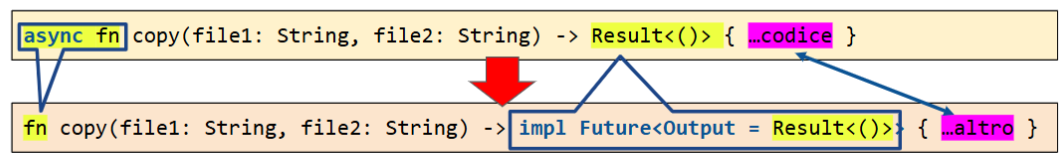
\includegraphics[width=0.3\linewidth]{content/API_Programming/images/2026-05-22-21-26-05.png}
% \end{figure}

% Se all'interno del codice della funzione è presente una chiamata ad un'altra
% funzione asincrona, per poter accedere al suo risultato occorre esplicitamente
% attenderlo, attraverso l'operatore \verb|.await|. Questo introduce un nuovo stato
% all'interno della macchina a stati associata alla funzione

% \begin{minted}[breaklines]{rust}
% async fn copy(h1: FileHandle, h2: FileHandle) -> std::io::Result<()> {
%   let mut buffer = vec![];
%   h1.read_async(&mut buffer).await?;
%   h2.write_async(&buffer).await
% }
% \end{minted}

\subsection{Un future è inerte: serve un esecutore}


\begin{center}
  \begin{minipage}{0.65\linewidth}
    Il compilatore genera i tipi della macchina a stati e riscrive le funzioni, ma il
    linguaggio si ferma qui. Nessun supporto precostituito per \textbf{eseguire} effettivamente i \textbf{Future}

    Affinché una computazione asincrona proceda, qualcuno deve farne avanzare la
    macchina a stati.
    Se viene chiamata una funzione async dentro un'altra funzione async, il suo Future viene
    automaticamente a far parte della macchina a stati del chiamante.
    Se viene chiamata da una funzione normale, occorre gestire il Future esplicitamente con un executor

    L'executor è uno \textbf{schedulatore cooperativo} a livello applicazione
    Mantiene i task pronti e ne fa avanzare la macchina a stati invocando il metodo \verb|poll()| del \verb|Future|.
    A differenza dello scheduler del S.O. non può sottrarre il controllo ad un task, che deve cederlo
    spontaneamente ad un punto di attesa (\verb|.await|)

  \end{minipage}%
  \hfill
  \begin{minipage}{0.3\linewidth}
    \centering
    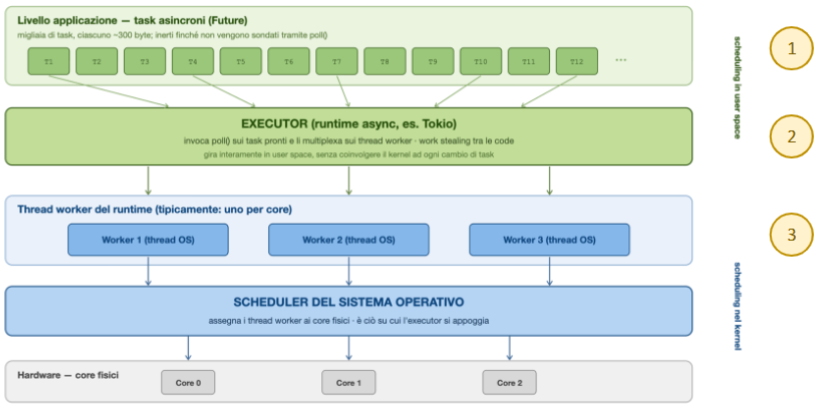
\includegraphics[width=\linewidth]{content/API_Programming/images/2026-05-25-12-45-24.png}
  \end{minipage}
\end{center}



\section{Il tratto Future}

Tratto che viene implementato dagli oggetti che descrivono una computazione
asincrona. Tale computazione può essere ancora in corso o essere terminata.

Il tratto offre un singolo metodo, \verb|poll(...)|, che implementa la logica della
macchina a stati associata alla funzione.
L'oggetto che implementa il tratto mantiene al suo interno lo stato corrente.

I metodo \verb|poll(...)| restituisce enum che può assumere due soli valori:
\begin{itemize}
  \item \verb|Poll:Pending| - per indicare che la computazione è ancora in corso
  \item \verb|Poll:Ready(T)| - per indicare che la computazione è terminata e ha come risultato \textbf{val}
\end{itemize}

Un oggetto che implementa questo tratto è \textbf{inerte}.
Affinché la computazione proceda, occorre che qualcuno ne invochi il metodo \verb|poll(...)|.



\begin{center}
  \begin{minipage}{0.65\linewidth}
    \begin{minted}[breaklines]{rust}
use std::pin::Pin;
use std::task::{Context, Poll};

pub trait Future {
  type Output;

  fn poll(self: Pin<&mut Self>, cx: &mut Context)
    -> Poll<Self::Output>;
}
    \end{minted}
  \end{minipage}%
  \hfill
  \begin{minipage}{0.3\linewidth}
    \begin{minted}[breaklines]{rust}
pub enum Poll<T> {
  Ready(T),
  Pending,
}
\end{minted}
  \end{minipage}
\end{center}

\verb|Pin<T>| è un particolare smart pointer che impedisce che la struttura venga mossa.
Permettendo l'uso di riferimenti relativi.


\verb|Context| incapsula un oggetto di tipo \textbf{Waker}, mediante il quale è possibile
notificare all'esecutore che il metodo \textbf{poll(...)} può essere richiamato.


\subsection{Chi invoca poll(): executor, reactor, Waker}

L'\textbf{executor} mantiene la coda dei task pronti e ne invoca il metodo \textbf{poll()} in un ciclo.
Se \textbf{poll()} restituisce \verb|Pending|, l'executormette il task da parte e passa al successivo.

Comportamento cooperativo, non preemptive: un task che non raggiunge mai \textbf{.await} monopolizza
il worker

\paragraph{Il problema:} come sa l'executor quando riprovare, senza fare polling attivo a vuoto?


\paragraph{Risposta}
Il \textbf{Waiker} contenuti nel \textbf{Context}.

\begin{itemize}
  \item Prima di restituire \textbf{Pending}, il \textbf{Future} registra il proprio \textbf{Waker} presso il sottosistema (es, il reactor
        I/O)
  \item Il reactor osserva gli eventi del sistema operativo (epoll ,kqueue, IOCP via mio)
  \item Quando l'evento atteso si verifica, il reactor risveglia il task, chiamando \textbf{wake()} sul \textbf{Walker}
  \item Il task torna nella coda dei pronti e l'executor lo ri-campiona: la macchina a stati avanza
\end{itemize}

È un modello ad eventi: non vengono sprecati cicli di CPU durante le attese








\section{Esecutori}

% Chi invoca una funzione asincrona, ottiene come risultato un \textbf{Future} nel proprio
% stato iniziale.
% Affinché possa capitare qualcosa, occorre che ne venga invocato il metodo \verb|poll(...)|.

% Se la funzione asincrona è chiamata all'interno di un'altra funzione asincrona,
% diventa automaticamente parte della macchina a stati del chiamante.

% Come succede per le funzioni \verb|read_async| e \verb|write_async|, mostrate
% nell'esempio, sarà responsabilità del chiamante della funzione esterna, gestire
% il \textbf{Future} risultante.

% Se si invoca una funzione asincrona all'interno di una funzione "normale", occorre
% gestire il risultato di tipo \textbf{Future} in modo esplicito, per farlo occorre
% disporre di un \textbf{Executor}.


% Se il compilatore supporta la generazione automatica dei tipi che implementano
% la macchina a stati associata ad una funzione asincrona e la riscrittura delle
% funzioni in modo opportuno, \textbf{nessun supporto} è invece offerto dal linguaggio per
% la gestione dell'esecuzione. Il programmatore può scegliere quale libreria
% adottare nel proprio progetto, in base alle specifiche necessità


Per far funzionare un programma Rust asincrono occorre aggiungere una libreria di
supporto all'esecuzione, a scelta del programmatore

% Sono disponibili diverse librerie alternative per questo scopo:
\begin{itemize}
  \item \textbf{Tokio} - la più diffusa: rete, file, timer, sincronizzazione, canali; basata sul crate
  \item \textbf{smol} - leggera, adatta a sistemi embedded
  \item \textbf{async-std} - controparte asincrona della libreria standard
\end{itemize}


% I diversi ambienti di esecuzione non sono equivalenti.
% \textbf{Tokio} implementa un ciclo reattivo proprio, basato sul crate ad alte prestazioni \textit{mio} (Metal I/O), che
% non è compatibile con i tratti usati dagli altri due.

Un runtime può basarsi su un singolo ciclo reattivo e/o utilizzare un thread-pool cui
delegare l'esecuzione di più \textbf{Future} in parallelo.
In questo caso, è possibile che l'elaborazione di una funzione asincrona inizi in un thread ma sia
continuata in un thread differente.
Questo implica che tutti i valori utilizzati nella funzione asincrona il cui uso si estende in più stati
devono implementare il tratto \textbf{Send}, mentre i riferimenti devono implementare il tratto \textbf{Sync}.


\section{Possesso nel tempo}

Nel codice sincrono, il possesso è legato prevalentemente allo stack corrente.
Nel codice asincrono, una computazione può sospendersi e riprendere più tardi.

Le variabili usate dopo \textbf{.await} diventano parte dello stato del \textbf{Future}.
Se l'esecutore è multithread, quel Future può essere spostato tra worker.


Nei programmi asincroni, il possesso attraversa il tempo, non solo lo spazio:

\begin{itemize}
  \item I dati usati dopo \textbf{.await} devono restare validi
  \item I task spostabili tra thread devono avere il tratto \textbf{Send}
  \item I riferimenti condivisi tra thread devono avere il tratto \textbf{Sync}
  \item La creazione di task indipendenti spesso richiede la proprietà dei dati
\end{itemize}

\section{Tokio: i costrutti di base}


% \section{Architettura di elaborazione}

% \begin{center}
%   \begin{minipage}{0.65\linewidth}
%     Tokio opera utilizzando un certo numero di
%     code di esecuzione (default: n° di core). Ogni coda è gestita da un ciclo reattivo
%     (Processor) che estrae ed esegue i task
%     presenti. Quando un Processor esaurisce i task della
%     propria coda, prova a rubarne alcuni ad altre
%     code, su base euristica. L'intero algoritmo è ottimizzato per ridurre al
%     minimo la sincronizzazione. Prevalentemente usando oggetti atomici.
%   \end{minipage}%
%   \hfill
%   \begin{minipage}{0.3\linewidth}
%     \centering
%     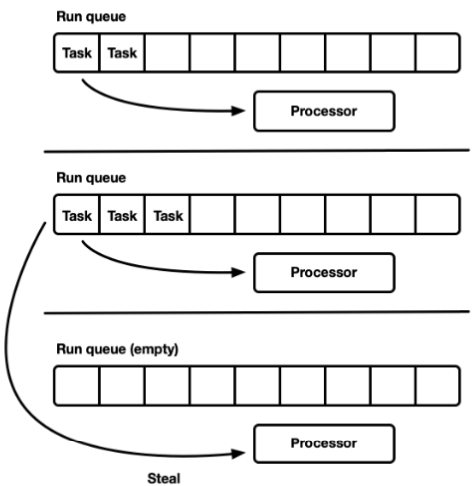
\includegraphics[width=0.6\linewidth]{content/API_Programming/images/2026-05-22-22-14-20.png}
%   \end{minipage}
% \end{center}

\subsection{Impostare un progetto con Tokio}
Si aggiunge \textbf{tokio} come dipendenza nel file Cargo.toml scegliendo quali
funzionalità attivare.

Si annota il punto di ingresso del programma con \verb|#[tokio::main]|, che avvia la libreria di
esecuzione e rende la funzione \textbf{main() async}

La proprietà \textbf{flavor} determina la struttura dell'esecutore:

\begin{itemize}
  \item \textbf{multi\_threaded} (dafault): un pool di thread worker, tipicamente uno per core
  \item \textbf{current\_thread}: un solo thread esegue tutti i task; utile per test e ambienti vincolati
\end{itemize}


\begin{minted}[breaklines]{rust}
# Cargo.toml
[dependencies]
tokio = { version = "1", features = ["full"] }

#[tokio::main(flavor = "multi_thread", worker_threads = 4)] //o altro…
async fn main() {
  //… creazione di future e attesa relativa
}
\end{minted}

\subsection{Attendere un Future: esecuzione sequenziale}

Il modo più semplice di usare un \textbf{Future} è attenderlo con \textbf{.await} dentro un blocco
\textbf{async}.

Due .await consecutivi creano una sequenza: il secondo parte solo quando il primo è completo.
Durante ogni attesa il thread è libero di servire altri task, ma questa funzione non avanza.
È il comportamento corretto quando il secondo passo dipende dal risultato del primo

\begin{minted}[breaklines]{rust}
async fn fetch_user(id:u64) -> User { /* … */ }
async fn fetch_orders(user: &User) -> Vec<Order> { /* … */ }

#[tokio::main]
async fn main() {
  let user = fetch_user(42).await; // prima questo…
  let orders = fetch_orders(&user).await; // …poi questo (dipende da user)
  println!("{} ha {} ordini", user.name, orders.len());
}
\end{minted}

\subsection{tokio::spawn - avviare task concorrenti}


\mintinline{rust}|tokio::spawn(future)| consegna un \textbf{Future}
all'esecutore come task indipendente.

A differenza di \textbf{.await},  l'esecuzione inizia subito e in modo concorrente, senza sospendere il
chiamate.

Restituisce un \textbf{JoinHandle}, che rappresenta il task e permette di ricuperarne il risultato


\paragraph{Vincoli sul tipo}

Il \textbf{Future} deve essere \textbf{Send} e \textbf{'static}:

\begin{itemize}
  \item \textbf{Send} perché il task può migrare tra i thread worker (work stealing)
  \item \textbf{'static} non vuol dire che i dati vivono per sempre, ma che non dipendono dallo stack corrente
  \item Si usa \textbf{move} per trasferire la proprietà dei dati al task
\end{itemize}

\textbf{.await} = "Aspetta questo $\Leftrightarrow$ = \textbf{spawn(...)} "fa' questo mentre faccio altro"


\begin{minted}[breaklines]{rust}
async fn expensive_io() -> Result<()> { /* … */ }
async fn do_other_work() { /* … */ }

#[tokio::main]
async fn main() {
  let h = tokio::spawn( async move { // parte immediatamente
    expensive_io().await // eseguito in background
  });

  do_other_work().await; // nel frattempo faccio altro
  let result = h.await.unwrap(); // quando ho finito, attendo il risultato
}
\end{minted}

\subsection{Non perdere il controllo dei task}

\textbf{spawn(...)} crea un task con un ciclo di vita separato.
Un task non osservato può:
\begin{itemize}

  \item Fallire senza che il chiamante se ne accorga
  \item Continuare oltre la richiesta che lo ha creato
  \item Complicare la terminazione e la cancellazione
\end{itemize}


Occorre conservare il valore di tipo \textbf{JoinHandle} restituito da \textbf{spawn(...)} quando
servono risultato, errore o arresto controllato.
Quando si hanno molti task omogenei è possibile usare strutture dedicate come
\textbf{JoinSet<T>}

\begin{itemize}
  \item Offre il metodo \textbf{spawn(...)} che automaticamente memorizza la \textbf{JoinHandle} corrispondente
  \item Permette di iterare su tutte le handle per attenderne la terminazione
\end{itemize}



% \begin{minted}[breaklines]{rust}
% tokio::task::spawn( f: T) -> JoinHandle<T::Output>
%   where T: Future + Send + 'static,
%   T::Output: Send + 'static
% \end{minted}

% Funzione che definisce un \textbf{task}, eseguito in modo concorrente con altri \textbf{task},
% la cui esecuzione inizia subito (a differenza di un \textbf{Future} di cui occorre invocare l'operatore \textbf{.await}).

% L'oggetto passato come parametro può essere il risultato dell'invocazione di una funzione async, o
% essere un blocco async passato per valore.

% \begin{minted}[breaklines]{rust}
% #[tokio::main]
% async fn main() {
%   let task = tokio::spawn(async { println!("Hello, Tokio!"); });
%   task.await.unwrap()
% }
% \end{minted}

% \subsection{Attendere la terminazione di più Future}
% La macro \mintinline{rust}|join!( f1: impl Future, …, fn: impl Future)|
% Può essere invocata all'interno di una funzione/blocco async e forza l'attesa fino a che tutti i
% suoi parametri non sono completati. Restituisce una tupla contenente i risultati associati ai suoi parametri.

% Una versione specializzata, \verb|try_join!(...)|, può essere usata quando le
% espressioni passate come parametro hanno come valore di ritorno \verb|Result<T,E>|.

% In questo caso viene restituito un oggetto \verb|Result| che contiene, se tutti i
% Future hanno avuto successo, una tupla con i relativi risultati, oppure, in
% corrispondenza del primo fallimento, l'errore corrispondente.

% \begin{minted}[breaklines]{rust}
% async fn do_stuff_async() { … }
% async fn more_async_work() { … }

% #[tokio::main]
% async fn main() {
%   let (first, second) = tokio::join!(
%   do_stuff_async(),
%   more_async_work()
%   );
%   // do something with the values
% }
% \end{minted}

\subsection{join! - attendere più Future insieme}


\mintinline{rust}|tokio::join!(f1, f2, ...)| attende il completamento di
\textbf{tutti i Future} passati.


\begin{itemize}
  \item Li fa progredire in modo interlacciato sullo stesso task: non viene eseguito spawn(), non viene richiesto il tratto Send
  \item Restituisce una tupla contenente i risultati, nell'ordine dei parametri passati
\end{itemize}

È il meccanismo corretto quando i compiti sono indipendenti e servono tutti i risultati

\mintinline{rust}|try_join!(...)| è la variante per \textbf{Future} che restituiscono
\textbf{Result<T,E>}.
Ritorna \textbf{Ok((r1, r2, ...))} se tutti hanno successo, oppure si interrompe al
\textbf{primo errore} restituendo

\begin{minted}[breaklines]{rust}
// Le due richieste non dipendono l'una dall'altra → attesa in parallelo
let (user, config) = tokio::join!(
fetch_user(42),
fetch_config()
);
// Variante con propagazione dell'errore
let (user, config) = tokio::try_join!(fetch_user(42), fetch_config())?;
\end{minted}


\subsection{select! - il primo che si completa}

\mintinline{rust}|tokio::select!(f1, f2, ...)| attende su più rami asincroni e procede con il
primo che termina. I rami non selezionati vengono \textbf{cancellati} ( viene invocato \textbf{Drop} sul loro \textbf{Future})

La sintassi di ogni ramo simile a quella di \textbf{match}:

\verb|<pattern> = <espressione async> (, if <guard>)? => <gestore>|

La guardia opzionale disattiva un ramo quando una precondizione è falsa

Un ramo \textbf{else} finale viene valutato se nessun ramo corrisponde al pattern indicato.

\begin{minted}[breaklines]{rust}
tokio::select! {
  data = fetch_from_network() => {
      process(data);
  },
  _ = tokio::time::sleep(Duration::from_secs(5)) => {
      eprintln!("timeout: nessuna risposta");
  }
}
\end{minted}

\subsection{Gestione del tempo}

\mintinline{rust}|tokio::time::sleep(d).await| sospende il task corrente per la durata indicata

\begin{itemize}
  \item Non consuma né CPU né un thread: occupa solo la memoria del \textbf{Future} (~ 300 byte)
  \item Allo scadere, l'esecutore risveglia il task e l'esecuzione riprende
\end{itemize}

\mintinline{rust}|tokio::time::timeout(d, future).await| impone un limite di tempo a
qualsiasi \textbf{Future}

\begin{itemize}
  \item Restituisce \verb|Result<T, Elapsed>: Ok(t)| se l'operazione completa in tempo, \textbf{Err} se scade prima
  \item È implementato tramite una select! tra il \textbf{Future} e un timer
\end{itemize}

\subsection{Cancellare un task}

La struct \textbf{JoinHandle} restituita da \textbf{spawn(...)}
offre il metodo \textbf{abort()} per
cancellare il task.


La cancellazione ha effetto quando il task è sospeso su \textbf{.await}.
Se il task è dentro un ciclo attivo, l'interruzione avviene al prossimo \textbf{.await}.

Invoca \textbf{abort()} si attende la \textbf{JoinHandle} per verificare
l'effettivo arresto. Si ottiene un \textbf{JoinError} con \verb|is\_cancelled() == true|

\begin{minted}[breaklines]{rust}
let handle = tokio::spawn(async {
  tokio::time::sleep(Duration::from_secs(10)).await;
});
// richiede la cancellazione
handle.abort();
// verifica che sia avvenuta
assert!(handle.await.unwrap_err().is_cancelled());
\end{minted}

\subsection{Esempio}



\begin{minted}[breaklines]{rust}
async fn count(){
  for i in 1..10 {
    tokio::time::sleep(Duration::from_secs(1)).await;
    println!("Count: {}", i);
  }
}

#[tokio::main]
async fn main() {
  let f1 = count();
  let f2 = async {
      for i in 'a'..='z' {
      tokio::time::sleep(Duration::from_millis(200)).await;
      print!("Main: {}", i);
      std::io::stdout().flush().unwrap();
    }
  };

  // f1 e f2 procedono in parallelo
  // AND
  tokio::join!(f1, f2); 

  // se voglio capire quale dei due termina per primo
  // interrompendo l'altro!
  // OR
  tokio::select! {
    _ = f1 => println!("f1 ha terminato"),
    _ = f2 => println!("f2 ha terminato"),
  };
}
\end{minted}


\section{Guida alla progettazione}

Quale costrutto, in quale situazione

\begin{table}[h!]
  \renewcommand{\arraystretch}{1.6}
  \centering
  \begin{tabularx}{\textwidth}{X X}
    \toprule
    Il lavoro è CPU intensive ($> \sim 100\mu$s) ?        & $\rightarrow$ Thread o Rayon                                          \\
    Passi di I/O che dipendono l'uno dall'altro?          & $\rightarrow$ \texttt{.await} in sequenza                             \\
    Avviare un'attività indipendente / cancellabile?      & $\rightarrow$ \texttt{tokio::spawn} $\rightarrow$ \texttt{JoinHandle} \\
    Più attività indipendenti, servono tutti i risultati? & $\rightarrow$ \texttt{tokio::join!} / \texttt{try\_join!}             \\
    Reagire alla prima tra N condizioni?                  & $\rightarrow$ \texttt{tokio::select!}                                 \\
    Passare dati tra task?                                & $\rightarrow$ canali (vedi oltre)                                     \\
    Stato mutabile condiviso tra task?                    & $\rightarrow$ \texttt{Arc<tokio::sync::Mutex<T>>}                     \\
    \bottomrule
  \end{tabularx}
\end{table}

\subsection{Esempio: sequenza o concorrenza?}
Lo stesso problema, due strutture diversa, in base alle \textbf{dipendenze tra i passi}

\begin{flushleft}
  \begin{minipage}[t]{0.45\linewidth}
    \raggedright
    \begin{minted}[breaklines]{rust}
// Dipendenti -> sequenza

// orders dipende da user
let user = fetch_user(id).await;
let orders = fetch_orders(&user).await;
// Tempo: t_user + t_orders
\end{minted}
  \end{minipage}%
  \hfill
  \begin{minipage}[t]{0.45\linewidth}
    \raggedright
    \begin{minted}[breaklines]{rust}
// Indipendenti -> concorrenza

// nessuna dipendenza tra i due
let (user, cfg) = tokio::join!(
  fetch_user(id),
  fetch_cfg()
);
//Tempo: max(t_user, t_cfg)
\end{minted}
  \end{minipage}
\end{flushleft}

Regola pratica: si introducono \textbf{.await} sequenziali solo quando un passo usa un
risultato precedente.
Se due operazioni sono indipendenti, \textbf{join!} le sovrappone senza creare task né richiedere
\textbf{Send}.

\subsection{Il caso speciale: attività che richiedono molta CPU}

La schedulazione implementata dall'esecutore è cooperativa

\begin{itemize}
  \item Un task async non deve occupare il thread soggiacente a lungo senza effettuare \textbf{.await}
  \item Un calcolo lungo ($>\,\sim 100\mu$s) senza punti di sospensione blocca il thread e ritarda tutti gli altri task su
        quella coda
  \item È l'errore più comune: "il mio server async è lento" spesso significa che un task non cede mai il
        controllo
\end{itemize}


\mintinline{rust}|tokio::task::spawn_blocking(f)| sposta una closure sincrona su un pool dedicato

Pool separato e limitato, distinto dai thread worker async.
Tokio mette a disposizione due thread pool: uno a dimensione fissa per gli executor, uno limitato per
le chiamate bloccanti. Per eseguire operazioni che richiedono un uso massiccio della CPU, si delega a librerie dedicate come
Rayon, eventualmente regolando la concorrenza con un semaforo


\subsection{Quattro modi di coordinate i Future}


\begin{table}[h!]
  \renewcommand{\arraystretch}{1.6}
  \centering
  \begin{tabular}{l l}
    \toprule
    \textbf{Caso}                    & \textbf{Strumento} \\
    \midrule
    Dipendenza                       & \texttt{.await}    \\
    Indipendenti, stessi scope       & \texttt{join!}     \\
    Indipendenti, lifecycle separato & \texttt{spawn}     \\
    Reagire al primo evento          & \texttt{select!}   \\
    \bottomrule
  \end{tabular}
\end{table}

\section{Condividere e comunicare}


\subsection{Architettura di elaborazione}




\begin{center}
  \begin{minipage}{0.65\linewidth}

    tokio opera utilizzando un certo numero di
    code di esecuzione (una per core).

    Ogni coda è gestita da un ciclo reattivo
    (Processor) che estrae ed esegue i task
    presenti.
    Quando un Processor esaurisce i task della
    propria coda, prova a rubarne alcuni ad altre
    code, su base euristica.
    Sincronizzazione minimizzata con operazioni
    atomiche

    \paragraph{Conseguenza:} un task può iniziare e
    proseguire su thread diversi → serve
    coordinamento.
    I valori che attraversano un \textbf{.await} devono essere \textbf{Send}
    I riferimenti condivisi devono essere \textbf{Sync}
    Stessa disciplina del multithread: i dati condivisi vanno protetti
  \end{minipage}%
  \hfill
  \begin{minipage}{0.3\linewidth}
    \centering
    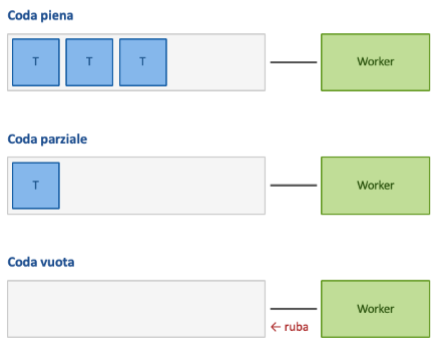
\includegraphics[width=\linewidth]{content/API_Programming/images/2026-05-25-14-17-50.png}
  \end{minipage}
\end{center}


\section{Condividere dati tra task}

Tokio mette a disposizione una ricca serie di primitive asincrone nel modulo
\textbf{tokio::sync}.

Due approcci:

\begin{itemize}
  \item Condivisione dello \textbf{stato} tramite \textbf{Barrier}, \textbf{Mutex}, \textbf{Notify}, \textbf{RwLock}, \textbf{Semaphore}
  \item Comunicazione tramite \textbf{messaggi} con canali  \textbf{oneshot}, \textbf{mpsc}, \textbf{broadcast}, \textbf{watch}
\end{itemize}

Sebbene assomiglino alle primitive della libreria standard, c'è una differenza
fondamentale:

\begin{itemize}
  \item Le operazioni di sincronizzazione sono \textbf{asincrone} e non bloccanti
  \item Se la risorsa non è disponibile, il task corrente viene sospeso fino a che non diventa possibile
        proseguire, senza impedire al thread soggiacente di elaborare altri task.
\end{itemize}




% \section{Selezionare il primo Future che si completa}

% La macro \verb|select!( ... )| permette di attendere su più rami asincroni,
% eseguiti nell'ambito dello stesso thread, quello che termina per primo.ù
% Cancellando l'esecuzione dei restanti. Può essere usata solo all'interno di
% funzioni/blocchi asincroni. Al suo interno è possibile inserire condizioni
% della forma.

% \mintinline{rust}|<pattern> = <async expression> (, if <precondition>)? => <handler>|
% \mintinline{rust}|else => <expression>|

% Il ramo \textbf{else}, se presente, viene valutato solo se nessuno dei rami precedenti ha avuto successo


% \begin{minted}[breaklines]{rust}
% async fn do_stuff_async() { … }
% async fn more_async_work() { … }

% #[tokio::main]
% async fn main() {
%   tokio::select! {
%     _ = do_stuff_async() => {
%       println!("do_stuff_async() completed first")
%     }
%     _ = more_async_work() => {
%       println!("more_async_work() completed first")
%     }
%   };
% }
% \end{minted}

% \section{Cancellare un task}

% \subsection{Metodo spawn}

% Il metodo \mintinline{rust}|tokio::spawn(...)| restituisce un valore di tipo \textbf{JoinHandle}.
% Esso offre il metodo \textbf{abort()} che permette la cancellazione del task, a condizione che esso sia in
% attesa su un qualche \textbf{Future}.
% Se, viceversa, il task sta è occupato in un ciclo di elaborazione attiva, la cancellazione avrà effetto nel
% momento in cui il task invocherà l'operatore \textbf{await}.
% Qualora \textbf{abort()} venisse invocato su un task già terminato, esso non avrà alcun effetto

% \subsection{Metodo Abort}
% L'invocazione di \textbf{abort()} è normalmente seguita da un'attesa sulla \textbf{JoinHandle}
% per verificare l'effettivo arresto del task.
% Se il task è stato effettivamente interrotto, verrà restituito un errore di tipo \textbf{JoinError} con
% l'indicazione dell'avvenuta cancellazione.
% Invocazioni multiple del metodo \textbf{abort()} hanno lo stesso effetto di una sola chiamata.

% Se il motore di esecuzione viene terminato, tutti i task ancora in corso sono
% automaticamente terminati.


% \begin{minted}[breaklines]{rust}
% let mut handles = Vec::new();
% for i in 1..4 {
%   handles.push(tokio::spawn(async move {
%     tokio::time::sleep(std::time::Duration::from_secs(10)).await;
%     i
%   }));
% }
% for handle in &handles {
%   handle.abort();
% }
% for handle in handles {
%   assert!(handle.await.unwrap_err().is_cancelled());
% }
% \end{minted}

% \section{Gestione del tempo}

% La funzione \mintinline{rust}|tokio::time::sleep(d: Duration).await| sospende
% l'esecuzione del task corrente per un tempo pari alla durata indicata. Durante
% l'attesa non viene consumata nessuna risorsa, se non la memoria necessaria a
% descrivere l'oggetto Future corrispondente. Allo scadere del tempo,
% l'esecuzione procede normalmente.


% La funzione \mintinline{rust}|tokio::time::timeout(d: Duration, f: F).await|
% attende per un tempo massimo pari alla durata indicata che il Future passato
% come secondo parametro si completi e restituisce un valore di tipo \verb|Result<T,Elapsed>|.
% Se l'esecuzione si completa in tempo, il risultato è positivo e
% contiene il valore restituito dal Future, altrimenti riporta un errore di tipo
% Elapsed

% \section{Eseguire compiti computazionalmente intensi}

% \begin{center}
%   \begin{minipage}{0.65\linewidth}
%     Se, in una funzione asincrona, occorre eseguire un compito computazionalmente
%     intenso, la cui durata possa superare il centinaio di microsecondi, è bene richiedere
%     che venga eseguito in un thread apposito.
%     Così da evitare di introdurre latenza nell'elaborazione degli altri task.
%     Si utilizza la funzione \mintinline{rust}|tokio::task::spawn_blocking(f: FnOnce()->R)|.
%   \end{minipage}%
%   \hfill
%   \begin{minipage}{0.3\linewidth}
%     \centering
%     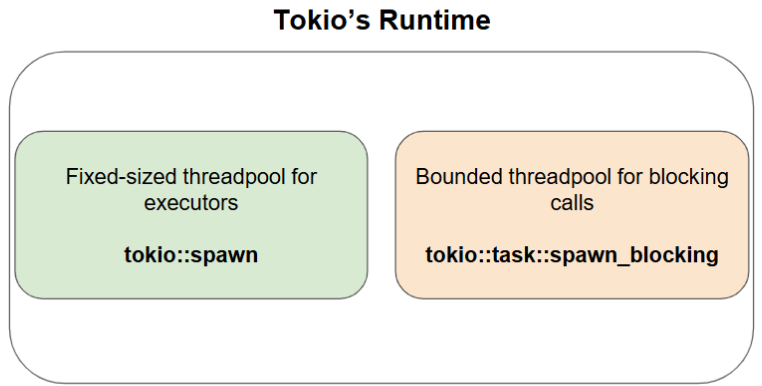
\includegraphics[width=\linewidth]{content/API_Programming/images/2026-05-22-22-48-25.png}
%   \end{minipage}
% \end{center}

% Occorre evitare di lanciare troppi task di questo tipo. Durante la loro
% esistenza, infatti, tenderebbero a richiedere l'uso di CPU introducendo contesa
% con i thread deputati a elaborare le code dei messaggi, aumentando la latenza
% complessiva del sistema. Può essere opportuno condizionarne l'esecuzione alla
% disponibilità di risorse globali (usando, ad esempio, un semaforo) o usare
% esecutori ad hoc, come quelli offerti dalla libreria \textbf{Rayon}.
% \section{Condividere dati tra task}

% Se due task hanno bisogno di condividere una struttura dati, questa deve essere
% opportunamente protetta. A seguito del meccanismo di \textit{work stealing} adottato
% dallo schedulatore, è infatti possibile che l'esecuzione avvenga in thread
% differenti. Occorre pertanto adottare le stesse precauzioni e strategie già
% viste con la programmazione \textit{multithread}.

% Tokio mette a disposizione una ricca serie di primitive asincrone nel modulo
% \verb|tokio::sync|
% Alcune basate sulla condivisione dello stato (\textbf{Barrier, Mutex, Notify, RwLock, Semaphore})
% Altre basate sulla comunicazione di messaggi (\textbf{canali oneshot, mpsc, broadcast, watch})


\subsection{Stato condiviso: Arc<tokio::sync::Mutex<T>>}

\begin{flushleft}
  \begin{minipage}[t]{0.35\linewidth}
    \raggedright

    Per condividere uno stato mutabile tra
    task, si combina \textbf{Arc} (possesso
    condiviso) con \textbf{Mutex} (accesso
    esclusivo).

    Si usa tokio::sync::Mutex, non std::sync::Mutex: il metodo lock() è asincrono.
    Attendere il lock con .await non blocca il thread: cede il controllo fino a che il lock è libero.
    Non mantenere un lock attraverso.await

  \end{minipage}%
  \hfill
  \begin{minipage}[t]{0.6\linewidth}
    \begin{minted}[breaklines]{rust}
use tokio::sync::Mutex;
use std::sync::Arc;
#[tokio::main]
async fn main() {
  let data = Arc::new(Mutex::new(0));
  let mut v = vec![];
  for _ in 0..4 {
    let data = Arc::clone(&data);
    v.push(tokio::spawn(async move {
      let mut lock = data.lock().await;
      *lock += 1;
    }));
  }
  for h in v { let _ = join!(h); }
  assert_eq!(*(data.lock().await), 4);
}
\end{minted}
  \end{minipage}
\end{flushleft}

\subsection{Stato condiviso vs canali}

Usare \textbf{Arc<Mutex<T>>} è semplice, ma spesso NON è la soluzione migliore


Può diventare:

\begin{itemize}
  \item Un collo di bottiglia
  \item Fonte di deadlock
  \item Difficile da far scalare
\end{itemize}

Stato condiviso $\Leftrightarrow$ sincronizzazione esplicita

Spesso è più semplice passare messaggi che condividere memoria

\begin{itemize}
  \item Elimina l'uso di lock
  \item Elimina corse critiche
  \item Struttura il flusso di comunicazione e di sincronizzazione allo stesso
        tempo
\end{itemize}


\begin{table}[h!]
  \renewcommand{\arraystretch}{1.6}
  \centering
  \begin{tabular}{ll}
    \toprule
    \textbf{Stato condiviso} & \textbf{Canali}                      \\
    \midrule
    Accesso diretto ai dati  & Comunicazione esplicita              \\
    Richiede lock            & Nessun lock                          \\
    Più flessibile           & Più strutturato                      \\
    Rischio deadlock         & Più sicuro                           \\
    Più difficile da scalare & Più naturale per sistemi concorrenti \\
    \bottomrule
  \end{tabular}
\end{table}

\begin{tcolorbox}
  \textbf{Note:} Preferire l'uso dei canali quando possibile
\end{tcolorbox}


\newpage
\subsection{Comunicare invece di condividere: i canali}

\begin{figure}[h!]
  \centering
  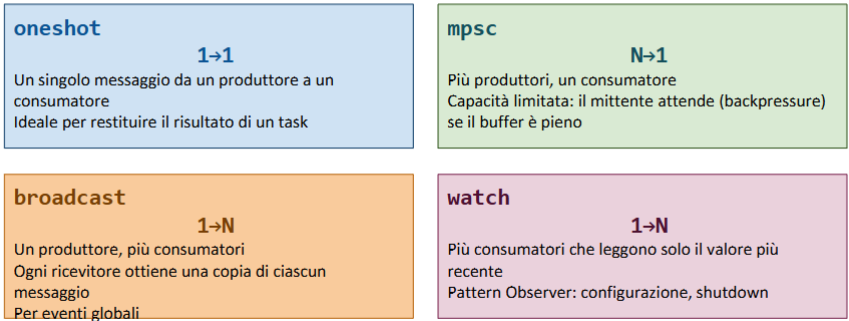
\includegraphics[width=0.7\linewidth]{content/API_Programming/images/2026-05-25-15-03-26.png}
\end{figure}



\subsubsection{Canali oneshot - Invio di un solo messaggio}

\begin{minted}[breaklines]{rust}
async fn some_computation() -> String { "Some result".to_string() }

#[tokio::main]
async fn main() {
let (tx, rx) = oneshot::channel();
  tokio::spawn(async move {
    let res = some_computation().await;
    tx.send(res).unwrap(); // il cananle viene chiuso automaticamente
  });
  // altro lavoro

  // attende il risultato
  let res = rx.await.unwrap();
}
\end{minted}

\subsubsection{Canali mpsc - Multiple Producer Single Consumer}

\begin{minted}[breaklines]{rust}
async fn some_computation(i: u32) -> String { format!("Value {}",i) }

#[tokio::main]
async fn main() {
  // capacità 10 → backpressure
  let (tx, mut rx) = mpsc::channel(10);

  tokio::spawn(async move {
    for i in 0..10 {
      let res = some_computation(i).await;
      tx.send(res).await.unwrap();
    }
  });
  while let Some(res) = rx.await.unwrap() { println!("{}", res); }
}
\end{minted}

\subsubsection{Canali broadcast - comunicazione molti-molti}

\begin{minted}[breaklines]{rust}
#[tokio::main]
async fn main() {
  let (tx, mut rx1) = broadcast::channel(16);
  let mut rx2 = tx.subscribe();

  tokio::spawn(async move {
  assert_eq!(rx1.recv().await.unwrap(), 10);
  assert_eq!(rx1.recv().await.unwrap(), 20);
  });
  tokio::spawn(async move {
  assert_eq!(rx2.recv().await.unwrap(), 10);
  assert_eq!(rx2.recv().await.unwrap(), 20);
  });
  tx.send(10).unwrap();
  tx.send(20).unwrap();
}
\end{minted}

\subsubsection{Canali watch - pattern Observer}
\begin{minted}[breaklines]{rust}
#[tokio::main]
async fn main() {
  let (tx, mut rx) = watch::channel("value 0");
  for i in 0..2 {
    let mut rx = rx.clone();
    tokio::spawn(async move {
      while rx.changed().await.is_ok() {
        println!("received: {:?}", *rx.borrow() );
      }
    });
  }
  let d = Duration::from_secs(1);
  tx.send("value 1").unwrap(); tokio::time::sleep(d).await;
  tx.send("value 2").unwrap(); tokio::time::sleep(d).await;
}
\end{minted}

\subsection{Backpressure}

Se i produttori sono più veloci dei consumatori, la coda cresce
Una coda illimitata trasforma un problema di throughput in un problema di
memoria.
Un canale limitato rende esplicita la capacità di un sistema.

Quando il buffer del canale è pieno, il produttore deve:

\begin{itemize}
  \item Attendere
  \item Scartare
  \item Degradare
  \item Fallire esplicitamente
\end{itemize}

\begin{tcolorbox}
  \textbf{Note:} La capacità non va nascosta: va progettata
\end{tcolorbox}

\subsection{Quando usare cosa}

\begin{table}[h!]
  \renewcommand{\arraystretch}{1.6}
  \centering
  \begin{tabular}{ll}
    \toprule
    \textbf{Caso}            & \textbf{Strumento}     \\
    \midrule
    Stato condiviso semplice & \texttt{Arc<Mutex<T>>} \\
    Pipeline / flusso dati   & \texttt{mpsc}          \\
    Notifica singola         & \texttt{oneshot}       \\
    Eventi globali           & \texttt{broadcast}     \\
    Stato osservabile        & \texttt{watch}         \\
    \bottomrule
  \end{tabular}
\end{table}

\subsection{Errori tipici in async Rust}

\begin{itemize}
  \item Usare async per lavoro CPU-bound
  \item Fare spawn e ignorare il JoinHandle
  \item Tenere il possesso di un lock mentre si esegue .await
  \item Usare Arc<Mutex<T>> come soluzione predefinita
  \item Usare code non limitate senza politica di backpressure
  \item Non prevedere timeout, cancellazione e terminazione del programma
\end{itemize}


\subsubsection{Implementare un semplice server Http}

\begin{minted}[breaklines]{rust}
use tokio::io::AsyncWriteExt;
use tokio::net::{TcpListener, TcpStream};
use tokio::task;

#[tokio::main]
async fn main() {
  let listener = TcpListener::bind("127.0.0.1:8181").await.unwrap();

  loop {
    let (stream, _) = listener.accept().await.unwrap();
    // ogni connessione -> un task indipendente
    tokio::spawn(handle_connection(stream));
  }
}

async fn handle_connection(mut stream: TcpStream) {
  let contents = "{\"message\": \"Hello, Tokio!\"}";

  let response = format!(
    "HTTP/1.1 200 OK\r\nContent-Type: application/json\r\nContent-Length:
    {}\r\n\r\n{}",
    contents.len(),
    contents
  );

  stream.write(response.as_bytes()).await.unwrap();
  stream.flush().await.unwrap();
}
\end{minted}

\section{Come funziona internamente}

\subsection{Esecuzione parziale}

La macchina a stati finiti può essere implementata da una chiusura.
Essa racchiude il proprio stato e tutte le variabili locali di cui l'esecuzione ha bisogno.
Quando viene eseguita ritorna un valore che indica se ha raggiunto uno degli stati finali o se si trova
ancora in uno stato intermedio.
Questo permette di non bloccare il thread corrente e procedere con l'esecuzione di altri task


I punti di blocco sono tutti in corrispondenza degli stati intermedi
Questi sono immediatamente preceduti dall'invocazione di una funzione asincrona.
Quando uno stato intermedio viene raggiunto, la chiusura ritorna


Perché la macchina a stati possa progredire occorrono due condizioni:
\begin{itemize}
  \item Che la funzione asincrona invocata scateni qualche attività (in che thread avviene?) che possa portare all'evoluzione dello stato
  \item Che ci sia qualcuno che indichi che vi sono le condizioni affinché lo stato possa evolvere
\end{itemize}



\subsection{Generare la macchina a stati}

\begin{minted}[breaklines]{rust}
async fn copy(h1: FileHandle, h2: FileHandle) -> std::io::Result<()> {
  let mut buffer = vec![];
  h1.read_async(&mut buffer).await?;
  h2.write_async(&buffer).await
}
\end{minted}

\begin{figure}[h!]
  \centering
  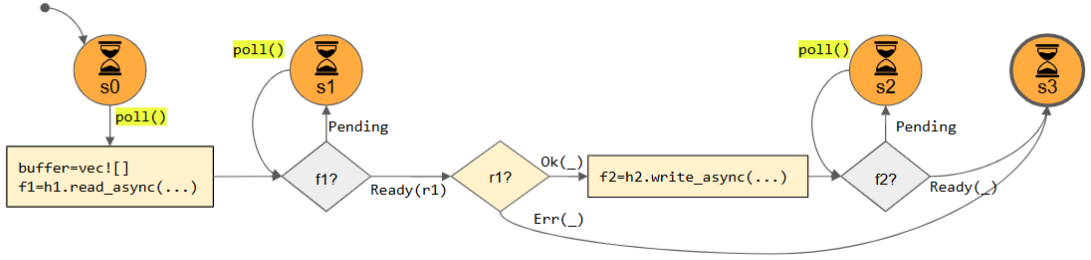
\includegraphics[width=0.45\linewidth]{content/API_Programming/images/2026-05-22-21-56-59.png}
\end{figure}

Per ciascuno stato individuato, il compilatore sintetizza una struct in cui
memorizzare le variabili locali necessarie per consentire l'esecuzione.

\begin{center}
  \begin{minipage}{0.47\linewidth}
    \begin{minted}[breaklines]{rust}
struct S0 {
  h1: FileHandle,
  h2: FileHandle,
}

struct S2 {
  f2: impl Future<Output=Result<usize>>,
}
\end{minted}
  \end{minipage}%
  \hfill
  \begin{minipage}{0.47\linewidth}
    \begin{minted}[breaklines]{rust}
struct S1 {
  h2: FileHandle,
  buffer: Vec<u8>,
  f1: impl Future<Output=Result<usize>>,
}

struct S3 {}
\end{minted}
  \end{minipage}
\end{center}


Inoltre genera una enum che racchiude i possibili stati e implementa il tratto Future

\begin{center}
  \begin{minipage}{0.37\linewidth}
    \begin{minted}[breaklines]{rust}
enum CopySM {
  s0(S0),
  s1(S1),
  s2(S2),
  s3(S3)
}
\end{minted}
  \end{minipage}%
  \hfill
  \begin{minipage}{0.6\linewidth}
    \begin{minted}[breaklines]{rust}
impl Future for CopySM {
  type Output = std::io::Result<()>
  fn poll(self: Pin<&mut Self>, cx: &mut Context)
                          -> Poll<Self::Output> {
  loop { match self {
  CopySM::s0(state) => { ... },
  CopySM::s1(state) => { ... },
  CopySM::s2(state) => { ... },
  CopySM::s3(state) => { ... },
  } }
  }
}
\end{minted}
  \end{minipage}
\end{center}

\begin{minted}[breaklines]{rust}
CopySM::s0(state) => {
  let mut buffer = vec![];
  let f1 = state.h1.read_async(&mut buffer);
  let state = S1 {h2: state.h2, buffer, f1 };
  *self = CopySM::S1(state);
}

CopySM::s1(state) => {
  match (state.f1.poll(cx) {
    Poll::Pending => return Poll::Pending,
    Poll::Ready(r1) =>
    if r1.is_ok() {
      let f2 = state.h2.write_async(&mut state.buffer);
      let state = S2{ f2 };
      *self = CopySM::s2(state);
    } else {
      *self = CopySM::s3(S3);
      return Poll::Ready(r1);
    }
  }
}

CopySM::s2(state) => {
  match (state.f2.poll(cx) {
    Poll::Pending => return Poll::Pending,
    Poll::Ready(r2) =>
      *self = CopySM::s3(S3);
      return Poll::Ready(r2);
  }
}

CopySM::s3(_) => {
  panic!("poll() was invoked again after Poll::Ready has been returned");
}
\end{minted}


\subsection{Implementare la funzione}

Il codice generato dal compilatore per la funzione si riduce
all'inizializzazione della macchina a stati.

\begin{minted}[breaklines]{rust}
fn copy(h1: FileHandle, h2: FileHandle) ->
            impl Future<Output = std::io::Result<()> > {
  CopySM::s0(
  S0 { h1, h2 }
  )
}
\end{minted}


\section{Prestazioni a confronto}

I costi di creazione e cambiamento di contesto tra attività asincrone e thread sono
analizzati nel sito

https://github.com/jimblandy/context-switch.
Il sito riporta la metodologia, il codice e i risultati ottenuti su un elaboratore
specifico, con il relativo sistema operativo. Gli ordini di grandezza sono comunque interessanti.

\begin{table}[h!]
  \renewcommand{\arraystretch}{1.5}
  \centering
  \begin{tabular}{l c c}
    \toprule
    \textbf{Operazione} & \textbf{async}   & \textbf{thread} \\
    \midrule
    Creazione di task   & $0.3 \mu s$      & $17 \mu s$      \\
    Cambio di contesto  & $0.2 \mu s$      & $1.7 \mu s$     \\
    Uso di memoria      & $300-500\,Bytes$ & $>9.5\,KBytes$  \\
    \bottomrule
  \end{tabular}
\end{table}

Dall'analisi di questi numeri, emerge che l'uso di costrutti asincroni può ridurre
l'utilizzo della memoria. Specialmente in quei contesti in cui si tenderebbe a preallocare un elevato numero di thread per poter
fare fronte a carichi di lavoro improvvisi (server di rete).

È meno oneroso creare task asincroni rispetto a thread. Inoltre il tempo necessario a cambiare contesto è minore, ma solo nei casi migliori: se il cambio di
contesto è dovuto alla disponibilità di dati su una periferica su cui si intende eseguire I/O, il costo è
analogo
Operazioni di I/O asincrone, che richiedano un'attesa, dovranno essere ritentate in
seguito. Questo richiede l'esecuzione di (almeno) due system-call, invece che una sola come nel caso sincrono

\subsection{Quando l'esecuzione asincrona non conviene?}


L'esecuzione asincrona non è universalmente migliore, ha un dominio di
applicazione preciso:

\begin{itemize}
  \item Compiti strettamente \textbf{legati alla CPU}: se i task non si
        sospendono quasi mai, async aggiunge complessità senza benefici; si usano i
        thread

  \item \textbf{Pochi compiti, di breve durata}: il costo dei thread è trascurabile e il codice sincrono è più semplice da
        scrivere e correggere

  \item Codice \textbf{fortemente sequenziale}: se non c'è nulla da sovrapporre, l'asincronicità è solo un
        appesantimento concettuale
\end{itemize}

L'esecuzione asincrona dà il meglio di sé quando si gestiscono \textbf{molte attese
  simultanee} come server di rete con migliaia di connessioni, client che interrogano molti servizi in parallelo, pipeline I/O-
intensive.

Si possono combinare i due mondi: una componente asincrona per I/O, \verb|spawn_blocking| o \verb|Rayon|
per il calcolo puro.





